\documentclass[10pt]{beamer}
% \documentclass[handout,10pt]{beamer}
\usepackage{my_style}

%%%%%%%%%%%%%%%%%%%%%%%%%%%%%%%%%%%%%%%%%%%%%%%%%%%%%%%%%%%%%%%%%%%%%%%%
\title[CS 357]{Lecture 16}
\subtitle{Monte Carlo}

\begin{document}
% -------------------------------------------------
\begin{frame}
  \titlepage
\end{frame}
% -------------------------------------------------
\begin{frame}{Goals}

We will answer these questions:
\begin{itemize}
    \item What are Monte Carlo simulations?
    \item How does Monte Carlo integration work?
    \item What are its advantages?
    \item What are its disadvantages?
\end{itemize}
    
\end{frame}

%%%%%%%%%%%%%%%%%%%%%%%%%%%%%%%%%%%%%%%%%%%%%%%%%%%%%%%%%%%%%%%%%%%%%%%%%
\sectionframe{Average Values}
%%%%%%%%%%%%%%%%%%%%%%%%%%%%%%%%%%%%%%%%%%%%%%%%%%%%%%%%%%%%%%%%%%%%%%%%
\begin{frame}{Continuous Function $y=f(x)$}
\begin{itemize}
        \define{Average Value}{
            The \textbf{average value} of a function $f:[a,b]\rightarrow \mathbb{R}$ is defined to be 
            $$av(f(x)) = f_{avg} = \frac{\int_a^b f(x)\,dx }{b-a}$$
        }
        \vspace{3mm}

    \item \textbf{Conceptually}, $f_{avg}$ it is the value you get \textit{on average} when you plug in a random number from $a$ to $b$ into $f(x)$\\[3mm]

    \item \textbf{Geometrically}, $y=f_{avg}$ is a line that marks the average height of $y=f(x)$ over $[a,b]$

\end{itemize}
\end{frame}
%%%%%%%%%%%%%%%%%%%%%%%%%%%%%%%%%%%%%%%%%%%%%%%%%%%%%%%%%%%%%%%%%%%%%%%%%
\begin{frame}{Example}
\begin{example}
Find the average value of $f(x) = 3x^2 + 1$ on $[0,2]$. 
\end{example}
\begin{itemize}
    \item By definition
    \begin{align*}
        f_{avg} &= \frac{\int_0^2 f(x) d x}{b-a} = \frac{(x^3 + x)|_0^2}{2-0} = \frac{10}{2} = 5\\ 
    \end{align*}
    \item Visual\\
        \begin{center}
        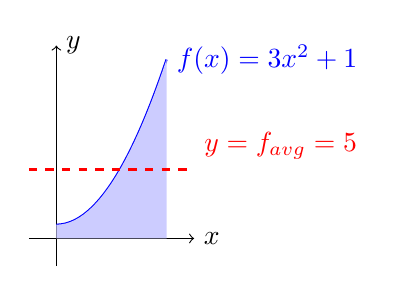
\begin{tikzpicture}[scale=0.7]
            % Define the function
            \def\func{(3*(\x)^2 + 1)/4}
        
            % Draw axes
            \draw[->] (-0.5, 0) -- (2.5, 0) node[right] {$x$};
            \draw[->] (0, -0.5) -- (0, 3.5) node[right] {$y$};
        
            % Plot the function
            \draw[domain=0:2, samples=100, smooth, thick, blue] plot ({\x}, {\func}) node[right] {$f(x) = 3x^2 + 1$};
        
            % Shade the area under the curve
            \fill[blue!20, domain=0:2, variable=\x]
                (0,0)
                -- plot ({\x}, {\func})
                -- (2, 0)
                -- cycle;
        
            % Draw the average value line
            \draw[dashed, red, thick] (-0.5,1.25) -- (2.5,1.25) node[above right] {$y = f_{\text{avg}} = 5$};
        \end{tikzpicture}
        \end{center}

\end{itemize}
\end{frame}
%%%%%%%%%%%%%%%%%%%%%%%%%%%%%%%%%%%%%%%%%%%%%%%%%%%%%%%%%%%%%%%%%%%%%%%%
\begin{frame}{Multivariable Functions}
    \begin{itemize}
        \define{Average Value for Scalar functions}{
            Let $f(X)$ be a function $f:\mathbb{R}^n\rightarrow \mathbb{R}$ defined on $D\in\mathbb{R}^n$. Then the \textbf{average value} of $f$ is
                $$av(f(X)) := f_{avg} := \frac{\int_D f(X)\,dX}{\mu(D)},$$
            where $\mu(D)$ is the \textbf{measure} of $D$.
        }
        \vspace{3mm}
        \item Conceptually, $f_{avg}$ is the average value obtained when plugging in a random point on $D$
        \item The average value can be defined for \textit{any} scalar-valued function
        \item The measure of a set is the length, area, or volume of the set
        \begin{itemize}
            \item $\mu( [3,7])= 7-3=4$
            \item $\mu( [a,b]\times[c,d] ) = (b-a)(d-c)$
            \item $\mu( \{x^2 + y^2 +z^2 < 1\} ) = 4/3 \pi r^3$
        \end{itemize}
    \end{itemize}
\end{frame}

% \begin{frame}{Integral example 1}
% There are many instances where the function is not so clear: \bigskip

%   \begin{itemize}
%     \item Goal: the average ``daily'' snowfall in Albuquerque last year
%     \item Function $s(day)$: snowfall on a particular day
%     \item Domain size: year (1D time interval)
%     \item Integration variable: day
%   \end{itemize}
% \begin{equation*}
%   average = \frac{\int_{day\in year}\; s(day)\; d_{day}}{length\; of\; year}
% \end{equation*}
% \end{frame}
% %%%%%%%%%%%%%%%%%%%%%%%%%%%%%%%%%%%%%%%%%%%%%%%%%%%%%%%%%%%%%%%%%%%%%%%%
% \begin{frame}{Integral example 2}
% In this example, you may not have access to data in every location: \bigskip
%   \begin{itemize}
%     \item Goal: the average snowfall in NM
%     \item Function $s(location)$: snowfall depending on $(x,y)$ location
%     \item Domain: NM (2D surface)
%     \item Integration variable: $(x,y)$ location
%   \end{itemize}
% \begin{equation*}
%   average = \frac{\int_{location\in NM}\; s(location)\; d_{location}}{area\; of\; NM}
% \end{equation*}
% \end{frame}
% %%%%%%%%%%%%%%%%%%%%%%%%%%%%%%%%%%%%%%%%%%%%%%%%%%%%%%%%%%%%%%%%%%%%%%%%%
% \begin{frame}{Integral example 3}
% Another real-world average that we may be interested in: \bigskip
%   \begin{itemize}
%     \item Goal: the average snowfall over NM for any arbitrary day
%     \item Function $s(location,\; day)$: snowfall depending on location and day
%     \item Domain: NM $\times$ year (2D space $\times$ time, or 3D)
%     \item Integration variable: location and day
%   \end{itemize}
% \begin{equation*}
%   average = \frac{\int_{day\in year}\int_{location\in NM}\; s(location,\; day)\; d_{location,day}}{area\; of\; NM \cdot length\; of\; year}
% \end{equation*}
% \end{frame}

\begin{frame}{Practical Applications of Average Values}
    \begin{enumerate}
        \item \textbf{Snowfall:} $s(location, day)$.
        \begin{itemize}
            \item $location$ = $(x, y)$ coordinates over NM.
            \item $day$ = day in a year.
            \item $av(s) = $ average snowfall over all of NM on any day of the year.
        \end{itemize}

        \item \textbf{Option Pricing:} $f(S_1, S_2, \ldots, S_n)$.
        \begin{itemize}
            \item $S_i$ = price of asset $i$ at maturity.
            \item $n$ = number of underlying assets.
            \item $av(f) = $ expected payoff of the option, integrated over all asset price combinations.
        \end{itemize}

        \item \textbf{Risk Assessment:} $f(X_1, X_2, \ldots, X_n)$.
        \begin{itemize}
            \item $X_i$ = uncertain parameter (e.g., material property, load condition).
            \item $n$ = number of parameters.
            \item $av(f) = $ probability of system failure, integrated over all uncertain parameters.
        \end{itemize}

        \item \textbf{Portfolio Optimization:} $f(w_1, w_2, \ldots, w_n)$.
        \begin{itemize}
            \item $w_i$ = weight of asset $i$ in the portfolio.
            \item $n$ = number of assets.
            \item $av(f) = $ expected portfolio return or risk, averaged over all possible allocations.
        \end{itemize}
    \end{enumerate}
\end{frame}
%%%%%%%%%%%%%%%%%%%%%%%%%%%%%%%%%%%%%%%%%%%%%%%%%%%%%%%%%%%%%%%%%%%%%%%%
\begin{frame}{High-dimensional Integration}

\begin{itemize}
    \item For many practical applications we must approximate 
        $$\int_D  f(X)\,dX $$
        where $X$ is a \textbf{high-dimensional variable}\\[5mm]

    \item We have only discussed quadratures for when $X$ is \textbf{one-dimensional }
        $$ \int_D f(X)\,dx = \int_a^b f(x)\,dx \approx \sum_i \alpha_i f(x_i)$$

    \begin{block}{Goal}
        We will learn a new easy way to integrate which works for \textit{any} dimensions.
    \end{block}
\end{itemize}
    
\end{frame}


%%%%%%%%%%%%%%%%%%%%%%%%%%%%%%%%%%%%%%%%%%%%%%%%%%%%%%%%%%%%%%%%%%%%%%%%
\sectionframe{Random Variables}
%%%%%%%%%%%%%%%%%%%%%%%%%%%%%%%%%%%%%%%%%%%%%%%%%%%%%%%%%%%%%%%%%%%%%%%%
\begin{frame}{Discrete Random Variables}

{\define{Discrete Random Variable}{
    A \textbf{discrete random variable} \(X\) takes values in a \textit{finite} set \(\{ x_0, x_1, \ldots, x_n \}\) with probabilities \(p_0, p_1, \ldots, p_n\), such that \(\sum_{i=0}^{n} p_i = 1\).
}}

\begin{itemize}
  \item $X$ is the \textbf{random variable}
  \item Outcomes: $X_0, X_1, \dots, X_n$
  \item Probabilities $p_0, p_1,\dots,p_n$ with $\sum_{i=0}^{n}p_i = 1$
  \item We write $P(X=X_0) = p_0$
\end{itemize}

\begin{block}{Example: Six-sided die}
\begin{itemize}
    \item $X =$ a roll of a die
    \item Outcomes: $x_1=1, x_2=2, \dots, x_6=6$
    \item Probability $P(X=4) = 1/6$
\end{itemize}

\end{block}  
\end{frame}
%%%%%%%%%%%%%%%%%%%%%%%%%%%%%%%%%%%%%%%%%%%%%%%%%%%%%%%%%%%%%%%%%%%%%%%%%
\begin{frame}{Expected Value and Variance}{The Discrete Case}

{\define{Discrete Statistics}{
  The \textbf{expected value} of a discrete random variable $x$ is
\begin{equation*}
  E[x] := \sum_{j=1}^{n}x_j p_j. 
\end{equation*}
The \textbf{variance} of $x$ is defined to be
\begin{equation*}
  \sigma^2[x] := E[(x-E[x])^2] % = E[x^2] - E[x]^2
\end{equation*}
}}

\begin{block}{Example: Six-sided die}
\begin{itemize}
  \item $E[x] = (1+2+\dots+6)/6 = 3.5$
  \item $\sigma^2[x] = (1/6)(1 - 3.5)^2 + (1/6)(2-3.5)^2 + ... + (1/6)(6 - 3.5)^2 = 2.916$
\end{itemize}
\end{block}  
\end{frame}

%%%%%%%%%%%%%%%%%%%%%%%%%%%%%%%%%%%%%%%%%%%%%%%%%%%%%%%%%%%%%%%%%%%%%%%%
\begin{frame}{Continuous Random Variable}

{\define{Continuous Random Variable}{
    A \textbf{continuous random variable} $X$ is a random quantity that can be an \textit{infinite} number of values and the probability of taking on a value is represented by a distribution $\rho(x)$.  
}}
\begin{itemize}
  \item Random variable range $X\in [a,b]$
  \item Probability: density function $\rho(x)$ with $\int_a^b
\rho(x)\,dx = 1$
  \item Probability is expressed with inequalities e.g. $P( X_1 > X)$
\begin{block}{Examples}
\begin{itemize}
    \item $X$ = Height of a person 
    \item $X$ = Shelf life of a product 
    \item $X$ = Time it takes to solve a puzzle 
\end{itemize}
    
\end{block}
\end{itemize}
\end{frame}

%%%%%%%%%%%%%%%%%%%%%%%%%%%%%%%%%%%%%%%%%%%%%%%%%%%%%%%%%%%%%%%%%%%%%%%%%

\begin{frame}{Expected Value and Variance}{The Continuous Case}

{\define{Continuous Statistics}{
\begin{itemize}
    \item The \textbf{expected value} of a continuous random variable $X$ is
    \begin{equation*}
      E[X] := \int_a^b x \rho(x) \,dx 
    \end{equation*}
    \item More generally, the expected value of $g(X)$ is 
    $$
        E[g(X)] := \int_a^b g(x) \rho(x)\,dx
    $$
    \item The \textbf{variance} of $X$ is defined to be
    \begin{equation*}
      \sigma^2[X] := E[(x-E[x])^2]  = \int_a^b (x-E[x])^2\rho(x)\,dx
    \end{equation*}
\end{itemize}
}}
\end{frame}

%%%%%%%%%%%%%%%%%%%%%%%%%%%%%%%%%%%%%%%%%%%%%%%%%%%%%%%%%%%%%%%%%%%%%%%%%

\begin{frame}{Uniform Random Variable}

    {\define{Uniform Random Variable}{
    A \textbf{uniform random variable} is a continuous variable that takes on a random number between $a$ and $b$ with equal probability. 
    }}
    \begin{itemize}
        \item By definition, if $X$ is uniform then the density function must be 
            $$\rho(x) = \frac{1}{b-a}$$
    \end{itemize}

    \begin{example}        
    
        Let \(a = 1\), \(b = 3\) (standard uniform distribution). Compute \(P(1.2 \leq X \leq 1.5)\):
    \end{example}
        \[
        P(0.2 \leq X \leq 0.5) = \int_{1.2}^{1.5} \frac{1}{3-1} \, dx = 0.15 = 15\% 
        \]



\end{frame}



%%%%%%%%%%%%%%%%%%%%%%%%%%%%%%%%%%%%%%%%%%%%%%%%%%%%%%%%%%%%%%%%%%%%%%%%%
\sectionframe{Monte Carlo Simulation}
%%%%%%%%%%%%%%%%%%%%%%%%%%%%%%%%%%%%%%%%%%%%%%%%%%%%%%%%%%%%%%%%%%%%%%%%%
\begin{frame}{Rolling a Die}

\begin{itemize}
    \item We may estimate the expected value of $X$, by drawing samples and taking the average
        \begin{equation*}
          E[x] =  \frac{1}{N} \sum_{j=1}^{N} x_i
        \end{equation*}
    \item Example - let $X$ be the outcome of a six-sided die
    
    \begin{block}{Estimated Average}
    \begin{itemize}
        \item 3 rolls: $3,1,6 \rightarrow E[x] \approx (3+1+6)/3 = 3.33$
        \item 9 rolls: $3,1,6,2,5,3,4,6,2 \rightarrow E[x] \approx (3+1+6+2+5+3+4+6+2)/9 = 3.51$
    \end{itemize}
    \end{block}
    
    \item As the number of rolls $N$ increases, we approach the true value $E[X]=3.5$
\end{itemize}
\end{frame}

%%%%%%%%%%%%%%%%%%%%%%%%%%%%%%%%%%%%%%%%%%%%%%%%%%%%%%%%%%%%%%%%%%%
\begin{frame}{Monte Carlo Simulation}

{\define{Monte Carlo Simulation}{
\textbf{Monte Carlo simulation} is a mathematical technique that uses repeated random sampling to estimate an outcome of a system with uncertain variables.
}}

\begin{itemize}
    \item Key Components
        \begin{itemize}
            \item Use knowledge of distribution of random variables in the sampling
            \item Increase repetition to reduce error and improve accuracy.
        \end{itemize}
    \item Applications:
        \begin{itemize}
            \item Estimating integrals (e.g., high-dimensional).
            \item Risk analysis and financial modeling.
            \item Simulating physical systems (e.g., particle dynamics, climate models).
        \end{itemize}
    \item Examples:
        \begin{itemize}
            \item Dice rolls 
            \item Coin flipping
        \end{itemize}
\end{itemize}

    
\end{frame}

%%%%%%%%%%%%%%%%%%%%%%%%%%%%%%%%%%%%%%%%%%%%%%%%%%%%%%%%%%%%%%%%%%%
\begin{frame}{Running a Simulation in Matlab}
    \begin{itemize}
        \item To simulate a dice roll, do 
            $$\texttt{X = randi(6)}$$
        \item To simulate a uniform random variable from 0 to 1, do 
            $$\texttt{X = rand}$$
        \item To simulate a coin toss (heads=1, tails=0) do 
            $$\texttt{X = (rand > 0.5)}$$
        \item To simulate a uniform random variable from $a$ to $b$, do 
            $$\texttt{X = (b-a)*rand + a}$$
    \end{itemize}
\end{frame}
%%%%%%%%%%%%%%%%%%%%%%%%%%%%%%%%%%%%%%%%%%%%%%%%%%%%%%%%%%%%%%%%%%%
\begin{frame}[fragile]{Simple Monte Carlo Example}
    \begin{example}
        On average, how many coin flips would it take to land 3 heads in a row?
    \end{example}

\begin{lstlisting}[mathescape]
flips_needed = zeros(1,100000);
for trial = 1:100000
    consecutive_heads = 0;
    flips = 0;
    while consecutive_heads < 3
        flips = flips + 1;
        if rand() < 0.5 % Simulate a coin flip 
            consecutive_heads = consecutive_heads + 1;
        else
            consecutive_heads = 0; % Reset if Tails
        end
    end
    flips_needed(trial) = flips;
end
average_flips = mean(flips_needed)
\end{lstlisting}
Output: \texttt{average\_flips = 14.0289} 
\end{frame}
%%%%%%%%%%%%%%%%%%%%%%%%%%%%%%%%%%%%%%%%%%%%%%%%%%%%%%%%%%%%%%%
\begin{frame}{The Real Answer?}
    \begin{example}
        On average, how many coin flips would it take to land 3 heads in a row?
    \end{example}
We model progress toward 3 consecutive heads using states:
\[
S_0:\text{ no streak},\qquad
S_1:\text{ 1 head},\qquad
S_2:\text{ 2 heads}.
\]
Let $E_0,E_1,E_2$ be the expected additional flips to reach 3 heads in a row.

\medskip

\begin{itemize}
    \item From $S_0$: 
    \[
      E_0=1+\tfrac12E_1+\tfrac12E_0 \;\Rightarrow\; E_0=2+E_1.
    \]
    \item From $S_1$:
    \[
      E_1=1+\tfrac12E_2+\tfrac12E_0.
    \]
    \item From $S_2$:
    \[
      E_2=1+\tfrac12E_0.
    \]
\end{itemize}
Solving the system gives:$E_0=14$. Monte Carlo would eventually give the same answer.

\end{frame}
%%%%%%%%%%%%%%%%%%%%%%%%%%%%%%%%%%%%%%%%%%%%%%%%%%%%%%%%%%%%%%%


\begin{frame}[fragile]{Average Value Example}
\begin{example}
    On average, what is the value of $f(x)=3x^2+1$ for a uniform random number  $x\in[0,2]$?
\end{example}

\begin{lstlisting}[mathescape]
fvals = zeros(1,100000);
f=@(x) 3*x^2 + 1;
for trial = 1:100000
    X = 2*rand; % random number on [0,2]
    fvals(trial) = f(X);
end
average_f = mean(fvals)
\end{lstlisting}
Output: \texttt{average\_f = 5.0005}\\
\vspace{3mm}
Notice how the output is close to $av(f) = 5$
\end{frame}


%%%%%%%%%%%%%%%%%%%%%%%%%%%%%%%%%%%%%%%%%%%%%%%%%%%%%%%%%%%%%%%%%%%
\begin{frame}{Law of Large Numbers}

\question{
    Why does Monte Carlo simulation work?
}


\begin{itemize}
    \item As $N \rightarrow \infty$, the error between the estimate and the true value is statistically zero.  
    \item That is, the estimate will converge to the correct value.  
    \item The probability $P(\cdot)$ is
        \begin{equation*} 
          P\left(E[x] = lim_{N\rightarrow\infty} \frac{1}{N} \sum_{i=1}^{N} x_i\right) = 1
        \end{equation*}
    \item This theoretical concept is called the \textbf{Law of Large Numbers}
    \item Increasing the number of trials eventually makes the error go to zero
\end{itemize}
\end{frame}

%%%%%%%%%%%%%%%%%%%%%%%%%%%%%%%%%%%%%%%%%%%%%%%%%%%%%%%%%%%%%%%%%%%%%%%%%
\sectionframe{Monte Carlo Integration}
%%%%%%%%%%%%%%%%%%%%%%%%%%%%%%%%%%%%%%%%%%%%%%%%%%%%%%%%%%%%%%%%%%%%%%%%
% \begin{frame}
% \frametitle{(Deterministic) Numerical integration}
% \begin{itemize}
%   \item Split domain into set of fixed segments
%   \item Sum function values, weighted by size of segments (Riemann!)
%   \item Is this like an expected value?  Perhaps $f(x_j)$ is the sampled value, and each value is ``equally" likely to occur.
% \end{itemize}
% \begin{center}
%   \pgfimage[height=4cm]{./figs/map2}
% \end{center}
% \end{frame}
%%%%%%%%%%%%%%%%%%%%%%%%%%%%%%%%%%%%%%%%%%%%%%%%%%%%%%%%%%%%%%%%%%%%%%%%%
\begin{frame}{Estimating $E[g(X)]$}

\begin{itemize}
    \item Suppose $X$ is a uniform random variable from $a$ to $b$

    \item Let $g(x)$ be some continuous real-value function $g:\mathbb{R}\rightarrow \mathbb{R}$

    \item By definition, the average value of $g(X)$ is exactly
    \begin{align*}
        E[g(X)] & = \int_a^b g(x)\rho(x)\,dx \\  
                & = \int_a^b g(x)  \left(\frac{1}{b-a}\right) \,dx \\  
                & = \frac{\int_a^b g(x)\,dx}{b-a}
    \end{align*}

    \item We can approximate $E[g(X)]$ with a Monte Carlo simulation
    \begin{align*}
        E[g(X)] & \approx \frac{1}{N} \sum_{i=1}^N g(x_i)
    \end{align*}
\end{itemize}
\end{frame}

%%%%%%%%%%%%%%%%%%%%%%%%%%%%%%%%%%%%%%%%%%%%%%%%%%%%%%%%%%%%%%%%%%%%%%%%
\begin{frame}{Connection Between Average Value and Integrals}

\begin{itemize}
    \item The average value of a function $E[f(X)]$ where $X$ is uniform on $[a,b]$ is 
        $$ E[f(X)]= \frac{1}{b-a}\int_a^b f(x)\,dx$$
    \item This is exactly equal to the average value of $f(x)$ for $a \le x \le b$ 
    \item Therefore, we have 
        $$ \int_a^b f(x)\,dx = (b-a)E[f(X)] = (b-a) f_{avg}$$
    \item Using Monte Carlo simulation we have 
        $$\int_a^b f(x)\,dx \approx (b-a) \frac{1}{N} \sum_{i=1}^N f(x_i) $$
\end{itemize}


    
\end{frame}

%%%%%%%%%%%%%%%%%%%%%%%%%%%%%%%%%%%%%%%%%%%%%%%%%%%%%%%%%%%%%%%%%%%%%%%%
\begin{frame}{Monte Carlo Integration}

    \begin{itemize}
        \item Using the Monte Carlo simulation we have the approximation 
            $$ \frac{\int_a^b g(x)\,dx}{b-a} \approx \frac{1}{N} \sum_{i=1}^N g(x_i)$$

        \item That means we have the following formula for the integral of $g(x)$:

            \begin{block}{Monte Carlo Integral Approximation}
                $$\int_a^b g(x)\,dx \approx \frac{b-a}{N} \sum_{i=1}^N g(x_i),$$
                where $x_i$ are random uniform variables on $[a,b]$.
            \end{block}
    \end{itemize}
    
\end{frame}


%%%%%%%%%%%%%%%%%%%%%%%%%%%%%%%%%%%%%%%%%%%%%%%%%%%%%%%%%%%%%%%%%%%%%%%%
\begin{frame}[fragile]{Monte Carlo Integration: Algorithm}
\begin{itemize}
    \item For uniform random numbers $x_1,\dots,x_n$, we have the numerical integration algorithm
\begin{equation*}
  \int_0^1 f(x)\,dx \approx \frac{1}{N} \sum_{i=1}^{N} f(x_i)  
\end{equation*}

\item The implementation in Matlab is very simple:
\begin{lstlisting}[mathescape]
n=100;
x=rand(n,1); % generate a vector of random numbers at once
a=f(x);
s=sum(a)/n;
\end{lstlisting}
\bigskip

\method{Monte-Carlo Integration}{Function $f(x)$, interval $[0,1]$, $N$ random points on $[0,1]$}{Approximation to $\int_0^1 f(x)\,dx$}{We can keep taking samples. The law of large numbers tells us this method converges. } 

\end{itemize}
\end{frame}
%%%%%%%%%%%%%%%%%%%%%%%%%%%%%%%%%%%%%%%%%%%%%%%%%%%%%%%%%%%%%%%%%%%%%%%%
\begin{frame}{Example for 1D}
\begin{example}
    Use Monte Carlo integration to approximate $f(x)=3x^2+1$ for $x\in[0,2]$. For the random variables $X$, use the values 
    $$ 0.1, 0.2, 1.2, 1.5.$$
\end{example}
\begin{itemize}
    \item  The approximation is 
        $$\int_0^2 f(x)\,dx \approx \frac{2-0}{4} \sum_{i=1}^4 f(x_i)$$
    \item Using the random numbers given, we have 
        \begin{align*}
            \int_0^2 f(x)\,dx &\approx \frac{1}{2} \sum_{i=1}^4 (3(x_i)^2 + 1)\\
                &=\frac{1}{2} \left[ 3(0.1)^2 + 3(0.2)^2 + 3(1.2)^2 + 3(1.5)^2 + 4  \right] = 7.61
        \end{align*}
\end{itemize}


\end{frame}



%%%%%%%%%%%%%%%%%%%%%%%%%%%%%%%%%%%%%%%%%%%%%%%%%%%%%%%%%%%%%%%%%%%%%%%%
\sectionframe{Two Dimensions}
%%%%%%%%%%%%%%%%%%%%%%%%%%%%%%%%%%%%%%%%%%%%%%%%%%%%%%%%%%%%%%%%%%%%%%%%
\begin{frame}{Two Dimensional Problem}

\begin{itemize}
\item Consider integrating the function of two variables
$$
  f(x,y) = 
\begin{cases}
1 & \quad (x,y)\in \, circle\\
0 & else
\end{cases}
$$
\item Let the domain of integration be the unit square $[0,1]^2$ 

\item Then the exact integral is just the area of the quarter circle
$$
  \int_0^1\int_0^1 f(x,y)\,dxdy = A =  \frac{\pi}{4}
$$
\end{itemize}
\begin{center}
  \pgfimage[height=4cm,width=4cm]{./figs/map4}
\end{center}
\end{frame}
%%%%%%%%%%%%%%%%%%%%%%%%%%%%%%%%%%%%%%%%%%%%%%%%%%%%%%%%%%%%%%%%%%%%%%%%%
\begin{frame}{Approximate $\pi$}

\begin{block}{Goal}
Knowing that 
$$
  \int_0^1\int_0^1 f(x,y)\,dxdy =   \frac{\pi}{4}
$$
use Monte Carlo integration to approximate the value of $\pi$.    
\end{block}
\vspace{5mm}
How?\\ 
\vspace{3mm}
\begin{itemize}
    \item Generate multiple random variables $X$ that are uniform in $[0,1]^2$
    \item Plug values of $X$ into $f$ and sum them 
    \item Divide sum by total number of points
    \item Multiply by 4 to get approximation of $\pi$
\end{itemize}
\begin{equation*}
  \pi \approx \frac{4}{N} \sum_{i=1}^{N}f(x_i,y_i)
\end{equation*}
\end{frame}
%%%%%%%%%%%%%%%%%%%%%%%%%%%%%%%%%%%%%%%%%%%%%%%%%%%%%%%%%%%%%%%%%%%%%%%%
\begin{frame}{The Dartboard Analogy}

\begin{enumerate}
    \item Throw $N$ darts randomly in $[0,1]^2$
    \item Count the number of darts that land inside $x^2+y^2 < 1$
    \item Divide total by $N$, then multiply by 4
\end{enumerate}
\begin{align*}
    \pi &\approx 4 \frac{\text{number of darts landed inside}}{\text{total darts thrown}}
\end{align*}
\begin{center}
  \pgfimage[height=4cm,width=4cm]{./figs/map3}
\end{center}
\end{frame}

%%%%%%%%%%%%%%%%%%%%%%%%%%%%%%%%%%%%%%%%%%%%%%%%%%%%%%%%%%%%%%%%%%%%%%%%
\begin{frame}[fragile]{Numerical Result}
\begin{lstlisting}[mathescape]
Input: $N$, seed
rng(seed) % set the seed
call rand in $2D$ to generate $(x_i, y_i)$
for $i$=1:$N$
    $sum = sum + f(x_i,y_i)$
end
$sum = 4*sum/N$
\end{lstlisting}

\begin{lstlisting}[mathescape]
Usage: monte_carlo_pi( niter, seed );

>>> monte_carlo_pi( 1000, 0 )
... estimate of pi is 3.132000000000000

>>> monte_carlo_pi( 10000000, 0 );
... estimate of pi is 3.14243...
\end{lstlisting}

\begin{itemize}
   \item $N=1000$ gives us 2 digits 
   \item $N=10,000,000$ gives us 4 digits
\end{itemize}

\end{frame}

%%%%%%%%%%%%%%%%%%%%%%%%%%%%%%%%%%%%%%%%%%%%%%%%%%%%%%%%%%%%%%%%%%%%%%%%%
\begin{frame}{Monte Carlo Convergence Rate}
The expected value of the \emph{error} is $\mO\left(\frac{1}{\sqrt{N}}\right)$
\begin{itemize}
  \item We are guaranteed this error by the law of large numbers
  \item Convergence does not depend on dimension
\end{itemize}
\bigskip 

\begin{block}{General Convergence}
The expected value of the \emph{error} in general for Monte Carlo integration is
   $$\mO\left(\frac{\sigma}{\sqrt{N}}\right)$$ where $\sigma$ is the standard
   deviation (square-root of the variance).
\end{block}
\end{frame}
%%%%%%%%%%%%%%%%%%%%%%%%%%%%%%%%%%%%%%%%%%%%%%%%%%%%%%%%%%%%%%%%%%%%%%%%
\begin{frame}{Disadvantage of Monte Carlo}
\begin{center}
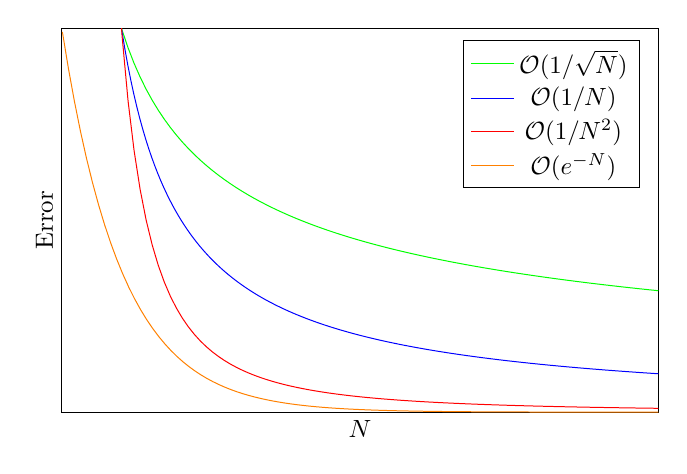
\begin{tikzpicture}[scale=0.9]
\begin{axis}[
    xlabel={$N$},
    ylabel={Error},
    xmin=0, xmax=10,
    ymin=0, ymax=1,
    legend pos=north east,
    grid=both,
    major grid style={line width=.2pt,draw=gray!50},
    width=10cm,
    height=7cm,
    xtick=\empty,
    ytick=\empty
]
\addplot[green,domain=0:10,samples=100] {1/sqrt(x)};
\addlegendentry{$\mathcal{O}(1/\sqrt{N})$}
\addplot[blue,domain=0:10,samples=200] {1/x};
\addlegendentry{$\mathcal{O}(1/N)$}
\addplot[red,domain=0:10,samples=100] {1/x^2};
\addlegendentry{$\mathcal{O}(1/N^2)$}
\addplot[orange,domain=0.01:10,samples=100] {exp(-x)};
\addlegendentry{$\mathcal{O}(e^{-N})$}
\end{axis}
\end{tikzpicture}
\end{center}

\begin{itemize}
    \item The main disadvantage of Monte Carlo is its \underline{slow} convergence rate
\end{itemize}
\end{frame}


%%%%%%%%%%%%%%%%%%%%%%%%%%%%%%%%%%%%%%%%%%%%%%%%%%%%%%%%%%%%%%%%%%%%%%%%%

\begin{frame}{Multidimensional extensions}
Why do care about a method that converges as slowly as $\mathcal{O}(\frac{1}{\sqrt{N}})$? \bigskip 
\begin{itemize}
  \item High-dimensional quadratures are difficult to derive 
  \item Many of the more sophisticated integration methods scale poorly with dimension
  \item Let $D$ be a difficult domain to integrate, e.g., complex geometry or high dimensionality
  \item Expected value
  \begin{align*}
  E[g(x)] & = \int_{x\in D} g(x)\rho(x)\,d x \approx \frac{1}{N} \sum g(x_i)
  \end{align*}

  
  \keyidea{
  \begin{itemize}
      \item Monte-Carlo is \textbf{robust} and\textbf{ easy to implement}
      \item Then convergence is \textbf{unaffected by the dimensionality} of the problem 
  \end{itemize}
  }
  
\end{itemize}
\end{frame}

%%%%%%%%%%%%%%%%%%%%%%%%%%%%%%%%%%%%%%%%%%%%%%%%%%%%%%%%%%%%%%%%%%%%%%%%%

\begin{frame}{Monte Carlo Summary}

        {\method{Monte Carlo Integration}{ $f:\mathbb{R}^n\rightarrow \mathbb{R}$}{Approximation to  $\int_D f(X)\,dX$}
        {Use random sampling to find the average value of $f$}
        }
        
        \begin{block}{Disadvantages}
        \begin{itemize}
            \item Slow convergence rate $\mO(N^{-1/2})$
        \end{itemize}
        \end{block}
        \begin{block}{Advantages}
        \begin{itemize}
            \item No increase in implementation difficulty w.r.t. dimension of $X$
            \item No slow down in convergence rate w.r.t. dimension of $X$
        \end{itemize}
        \end{block}

\end{frame}

\end{document}
